\documentclass[tikz]{standalone}
\usepackage{framed}
\usepackage{amsmath} 
\usepackage{amsfonts}
\DeclareMathOperator{\f}{f}
\usepackage{xcolor}

\usetikzlibrary{shadows.blur}
\usetikzlibrary{arrows}
\usetikzlibrary{positioning}

\begin{document}
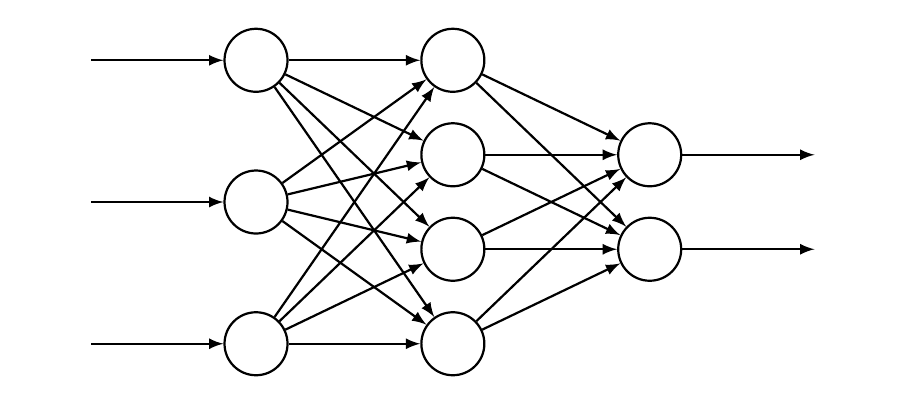
\begin{tikzpicture}[]
	%\draw[help lines] (-2,0) grid (20,10);
	
	\tikzstyle{vnode} = [circle,draw,thick,fill=white,minimum size=8mm]
	\tikzstyle{inode} = [minimum size=8mm]
	\tikzstyle{vedge} = [->,>=latex,thick]
	
	
	\node[inode] (ii1) at (-9, 0) {};
	\node[inode] (ii2) at (-9, -1.8) {};
	\node[inode] (ii3) at (-9, -3.6) {};
	
	\node[vnode] (i1) at (-6.5, 0) {};
	\node[vnode] (i2) at (-6.5, -1.8) {};
	\node[vnode] (i3) at (-6.5, -3.6) {};

	\node[vnode] (h1) at (-4, 0) {};
	\node[vnode] (h2) at (-4,  -1.2) {};
	\node[vnode] (h3) at (-4,  -2.4) {};
	\node[vnode] (h4) at (-4,  -3.6) {};
	
	\node[vnode] (o1) at (-1.5,  -1.2) {};
	\node[vnode] (o2) at (-1.5,  -2.4) {};

	\node[inode] (oo1) at (1, -1.2) {};
	\node[inode] (oo2) at (1, -2.4) {};

	\draw (ii1) edge [vedge] (i1);
	\draw (ii2) edge [vedge] (i2);
	\draw (ii3) edge [vedge] (i3);

	\draw (i1) edge [vedge] (h1);
	\draw (i1) edge [vedge] (h2);
	\draw (i1) edge [vedge] (h3);
	\draw (i1) edge [vedge] (h4);

	\draw (i2) edge [vedge] (h1);
	\draw (i2) edge [vedge] (h2);
	\draw (i2) edge [vedge] (h3);
	\draw (i2) edge [vedge] (h4);
	
	\draw (i3) edge [vedge] (h1);
	\draw (i3) edge [vedge] (h2);
	\draw (i3) edge [vedge] (h3);
	\draw (i3) edge [vedge] (h4);

	\draw (h1) edge [vedge] (o1);
	\draw (h1) edge [vedge] (o2);

	\draw (h2) edge [vedge] (o1);
	\draw (h2) edge [vedge] (o2);

	\draw (h3) edge [vedge] (o1);
	\draw (h3) edge [vedge] (o2);

	\draw (h4) edge [vedge] (o1);
	\draw (h4) edge [vedge] (o2);

	\draw (o1) edge [vedge] (oo1);
	\draw (o2) edge [vedge] (oo2);

\end{tikzpicture}
\end{document}
